\documentclass[12pt]{article}
\usepackage{ctex}
\usepackage{setspace}
\usepackage{float}
\usepackage{makecell}
\usepackage{booktabs}
\usepackage{multirow}
\usepackage{multicol}
\usepackage{array}
\usepackage{lastpage}
\usepackage{caption}
\usepackage[margin=1in]{geometry}%设置边距,符合Word设定
\usepackage{graphicx}%插入图片
\graphicspath{{Figures/}}%文章所用图片在当前目录下的 Figures目录

\title{专利名字}
\date{} %不显示日期

\usepackage{fancyhdr} % 设置页眉页脚
\pagestyle{fancy}
\renewcommand{\headrulewidth}{1pt} % 分隔线宽度
\renewcommand{\footrulewidth}{0pt}
\fancyfoot[C]{\thepage/\pageref{LastPage}}

\usepackage{hyperref} % 对目录生成链接,注:该宏包可能与其他宏包冲突,故放在所有引用的宏包之后
\hypersetup{
    colorlinks = true,  % 将链接文字带颜色
	hidelinks, % 隐藏连接样式
	allcolors=black,
	pdfstartview=Fit,
	breaklinks=true,
	bookmarksopen = true, % 展开书签
	bookmarksnumbered = true, % 书签带章节编号
	pdftitle = 专利名字, % 标题
	pdfauthor = xxx % 作者
    }

\begin{document}
\captionsetup{labelformat=default,labelsep=space} %去除题注的冒号

% 说明书摘要--------------------------------------------------------------
\fancyhead[C]{说明书摘要}
\section*{发明名称}
专利名字

\section*{摘要}
本发明公开了一种xxxxxxxxxxxxxxxxxxxxxxxxxxxxxxxxx

\hspace{2cm}
\begin{figure}[hbt]
	\centering
	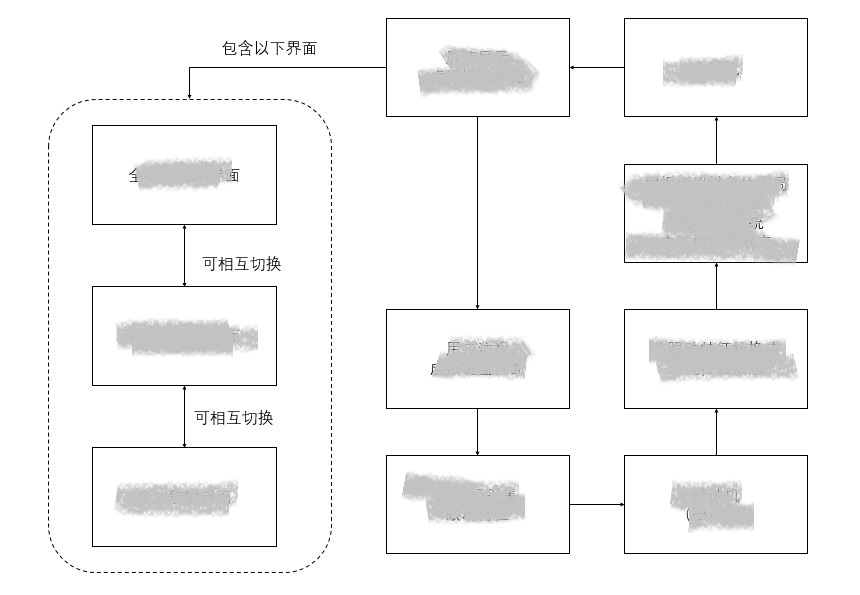
\includegraphics[width=16cm]{功能框图v2.jpg}
\end{figure}

\newpage
% 权利要求书--------------------------------------------------------------
\fancyhead[C]{权利要求书}
\section*{权利要求书}
1.一种xxxxxxxxxxxxxxxxxxxxxxxxxxxxxxxxxxxxxxxxxxx

\newpage
%专利说明书--------------------------------------------------------------
\fancyhead[C]{专利说明书}

\begin{center}
	\LARGE{专利名字}
\end{center}

\section*{技术领域}%小标题不带序号
本发明专利涉及一种xxxxxxxxxxxxxxxxxxxxxxxxxxxxxxxxxxx

\section*{背景技术}
现有的xxxxxxxxxxxxxxxxxxxxxxxxxxxxxxxxxxxxxxxxxx

而xxxxxxxxxxxxxxxxxxxxxxxxxxxxxxxxxxxxxxxxxxxxxx

现有的xxxxxxxxxxxxxxxxxxxxxxxxxxxxxxxxxxxxxxxxxxxxxxxxxxxxxxxx

现有的xxxxxxxxxxxxxxxxxxxxxxxxxxxxxxxxxxxxxxxxxxxxxxxxxxxxxxxxx

\section*{发明内容}
针对现有技术存在的缺陷,本发明基于
xxxxxxxxxxxxxxxxxxxxxxxxxxxxxxxxxxxxxxxxxxxxxxxxxxxxxxxxxxxxxxxx

为实现上述目的,本发明提供了如下技术方案:

~

xxxxxxxxxxxxxxxxxxxxxxxxxxxxxxxxxxxxxxxxxxxxxxxxxxxxxx

~

xxxxxxxxxxxxxxxxxxxxxxxxxxxxxxxxxxxxxxxxxxxxxxxxxxxxxx包括以下组成部分,

xxxxxxxxxxxxxxxxxxxxxxxxxxxxxxxxxxxxxxxxxxxxxxxxxxxxxxxxxxxxxxxxx

~

区别于现有技术,上述技术方案的有益效果如下:

1.xxxxxxxxxxxxxxxxxxxxxxxxxxxxxxxxxxxxxxxxxxxxxxxx

\newpage
\section*{附图说明}
图1是根据该系统的功能示例出的
xxxxxxxxxxxxxxxxxxxxxxxxxxxxxxxxxxxx

~

\section*{具体实施方式}
为了更好地说明本发明,现结合具体实施例以及说明书附图对技术方案作进一步的说明。
xxxxxxxxxxxxxxxxxxxxxxxxxxxxxxxxxxxxxxxxxxxxxxxx

\newpage
% 说明书附图--------------------------------------------------------------
\fancyhead[C]{说明书附图}
\begin{figure}[hbtp]
	\centering
	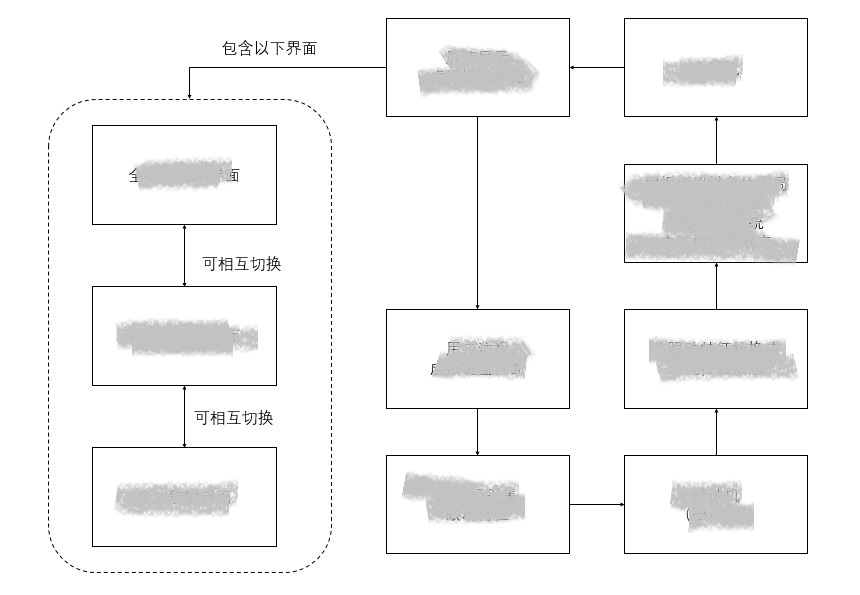
\includegraphics[width=16cm]{功能框图v2.jpg}
	\caption{}
\end{figure}

\end{document}